\documentclass[11pt,a4paper,twocolumn]{article}

% ============================================================================
% PACKAGES
% ============================================================================
\usepackage[utf8]{inputenc}
\usepackage[T1]{fontenc}
\usepackage{times}
\usepackage[margin=0.75in]{geometry}
\usepackage{graphicx}
\usepackage{booktabs}
\usepackage{hyperref}
\usepackage{amsmath,amssymb,amsfonts}
\usepackage{xcolor}
\usepackage{flushend}
\usepackage{caption}
\usepackage{subcaption}
\usepackage{algorithm}
\usepackage{algorithmic}
\usepackage{enumitem}
\usepackage{fancyhdr}
\usepackage{titlesec}
\usepackage{cite}
\usepackage{multirow}
\usepackage{tabularx}
\usepackage{tikz}
\usetikzlibrary{shapes.geometric, arrows.meta, positioning, fit, backgrounds, calc, decorations.pathreplacing}

% ============================================================================
% STYLE CONFIGURATION
% ============================================================================

\hypersetup{
    colorlinks=true,
    linkcolor=black,
    filecolor=black,
    urlcolor=blue,
    citecolor=black,
    pdfborder={0 0 0}
}

\titleformat{\section}{\large\scshape\bfseries}{\thesection}{1em}{}
\titleformat{\subsection}{\normalsize\bfseries}{\thesubsection}{1em}{}
\titleformat{\subsubsection}{\normalsize\itshape}{\thesubsubsection}{1em}{}
\titlespacing*{\section}{0pt}{1.5em}{0.75em}
\titlespacing*{\subsection}{0pt}{1.0em}{0.5em}
\titlespacing*{\subsubsection}{0pt}{0.8em}{0.4em}

\pagestyle{fancy}
\fancyhf{}
\fancyhead[C]{\small BALE: Graph-Based Contract Intelligence with Dispute Prediction}
\fancyfoot[C]{\thepage}
\renewcommand{\headrulewidth}{0pt}

% ============================================================================
% TITLE
% ============================================================================
\title{\vspace{-1cm}\huge\textbf{BALE: Graph-Based Contract Intelligence\\with Inter-Clause Conflict Detection\\and Dispute Hotspot Prediction}}

\author{
\large\textbf{Hamza Masmoudi}\\
\small Independent Researcher\\
\small\url{https://github.com/hamza2masmoudi/BALE-project}
}

\date{}

% ============================================================================
% DOCUMENT
% ============================================================================
\begin{document}

\twocolumn[
\maketitle
\begin{@twocolumnfalse}
\begin{abstract}
\noindent Automated contract analysis systems typically treat clauses as independent units, classifying each in isolation and aggregating risk scores through simple heuristics. This approach ignores a fundamental property of legal instruments: clauses interact. An indemnification provision may conflict with a liability cap; a data protection clause may be unenforceable without a corresponding confidentiality agreement. We present \textbf{BALE} (Binary Adjudication and Litigation Engine), a contract intelligence framework that models these inter-clause relationships explicitly through a \textit{Contract Reasoning Graph}.

BALE operates as a four-stage pipeline: (1)~zero-shot embedding classification using a multilingual sentence encoder, achieving \textbf{80.2\%} accuracy across English and French without fine-tuning; (2)~graph construction from a knowledge base of 16 legal doctrinal relationships encoding conflicts, dependencies, and constraints; (3)~power asymmetry detection that quantifies party-level obligation imbalance; and (4)~dispute hotspot prediction that localizes which specific clauses are most likely to be contested. V11 extends the pipeline with five innovations: semantic chunking via embedding-based boundary detection, Bayesian confidence calibration, a clause rewrite engine with 75 gold-standard templates, Monte Carlo risk simulation with uncertainty quantification, and cross-contract corpus intelligence for anomaly detection. Evaluated on 20 contracts (15 curated + 5 CUAD) spanning 7 contract types, the V11 pipeline achieves 100\% success rate at 296ms average latency, generating 79 rewrite suggestions and flagging 11 corpus anomalies across the evaluation corpus.

\vspace{0.8em}
\noindent\textbf{Keywords:} Legal NLP, Contract Analysis, Knowledge Graphs, Dispute Prediction, Multilingual Classification, Risk Assessment
\end{abstract}
\vspace{1.5em}
\end{@twocolumnfalse}
]

% ============================================================================
\section{Introduction}
% ============================================================================

Commercial contracts govern economic relationships estimated at trillions of dollars globally, yet their analysis remains largely manual~\cite{susskind2017}. The recent application of NLP to legal text has focused primarily on two tasks: clause extraction~\cite{hendrycks2021} and clause classification~\cite{chalkidis2020}. While these advances enable the identification of what type of clause appears in a contract, they do not address a more consequential question: \textit{how do clauses interact with each other, and where do those interactions create risk?}

Consider an indemnification clause that requires Party A to ``indemnify and hold harmless'' Party B against all claims. If the same contract contains a limitation of liability clause capping damages at the contract value, these two provisions are in direct tension: the indemnification promises unlimited protection while the liability cap restricts it. This conflict creates enforcement risk that no clause-level classifier can detect, because the risk emerges from the \textit{relationship} between clauses, not from either clause in isolation.

We identify three limitations of existing contract analysis systems:

\begin{enumerate}[leftmargin=*]
    \item \textbf{Clause Independence Assumption.} Current systems classify clauses independently, missing inter-clause conflicts, dependencies, and redundancies that determine enforceability.
    \item \textbf{Structural Blindness.} Risk is computed as an aggregate of per-clause scores, ignoring structural properties such as missing clauses, unsatisfied dependencies, and incomplete coverage.
    \item \textbf{Symmetry Blindness.} Standard classification provides no information about which party bears disproportionate risk, a critical factor in negotiation and dispute.
\end{enumerate}

To address these gaps, we introduce BALE, a contract intelligence framework built on three principles. First, we model the contract as a \textit{typed graph} where nodes are classified clauses and edges encode legal doctrinal relationships (conflicts, dependencies, constraints). Second, we detect \textit{power asymmetry} by analyzing the distribution of obligations and protections across parties. Third, we synthesize these signals into \textit{dispute hotspot predictions}: per-clause probabilities indicating where litigation is most likely to arise.

Our contributions are:
\begin{itemize}[leftmargin=*]
    \item A zero-shot embedding classifier that achieves 80.2\% overall accuracy across English and French without fine-tuning, running in under 5ms per clause.
    \item A Contract Reasoning Graph formalism encoding 16 inter-clause relationships derived from legal doctrine, enabling automated detection of conflicts, missing dependencies, and structural gaps.
    \item A dispute hotspot predictor that localizes risk to specific clauses rather than producing contract-level aggregates.
    \item Five V11 innovations: semantic chunking, Bayesian confidence calibration, a contrastive clause rewrite engine, Monte Carlo risk simulation, and cross-contract corpus intelligence.
    \item An empirical evaluation on 20 contracts with ablation studies demonstrating each component's contribution.
\end{itemize}

% ============================================================================
\section{Related Work}
% ============================================================================

\subsection{Legal NLP and Contract Understanding}

The application of NLP to legal documents has evolved from rule-based information extraction~\cite{wyner2010} to transformer-based approaches. The CUAD dataset~\cite{hendrycks2021} established a standard benchmark for contract clause extraction, defining 41 clause types across 510 contracts. Chalkidis et al.~\cite{chalkidis2020} introduced LegalBERT, a domain-adapted BERT model achieving strong performance on legal text classification. More recently, Chalkidis et al.~\cite{chalkidis2022} released LexGLUE, a multi-task benchmark for legal language understanding.

However, these approaches operate at the clause level: they identify and classify individual provisions without modeling how clauses relate to each other. ContractNLI~\cite{koreeda2021} introduced natural language inference for contracts but remains limited to entailment between a hypothesis and a single clause, rather than reasoning across the full contract structure.

\subsection{Graph-Based Document Analysis}

The use of graph representations for document understanding has shown promise in scientific literature~\cite{luan2018} and knowledge extraction~\cite{ji2022}. In the legal domain, knowledge graphs have been applied primarily to case law citation networks~\cite{zhong2020} and statute cross-referencing. Our work differs by constructing graphs \textit{within} a single document, where nodes are clauses and edges encode doctrinal relationships specific to contract law.

\subsection{Neuro-Symbolic Legal Reasoning}

Neuro-symbolic approaches combine neural perception with symbolic reasoning~\cite{garcez2019}. In legal AI, this has taken forms including logic-augmented neural training~\cite{ashley2017} and rule-based post-processing of neural outputs. Our architecture follows the latter paradigm: the neural component (embedding classifier) handles perception (clause classification), while the symbolic component (graph construction, power analysis) handles reasoning over the classified structure.

\subsection{Multilingual Legal NLP}

Cross-lingual transfer for legal text remains challenging due to the jurisdiction-specific nature of legal language~\cite{niklaus2021}. Prior work has relied on multilingual fine-tuning or parallel corpora. Our approach leverages a pretrained multilingual sentence encoder (paraphrase-multilingual-MiniLM-L12-v2), achieving strong French performance (85.0\%) without any French-specific fine-tuning, suggesting that legal clause semantics transfer well across languages at the embedding level.

% ============================================================================
\section{Methodology}
% ============================================================================

We define the contract analysis task as follows. Given a contract text $\mathcal{D}$, the system must produce: (a) a typed classification $y_i$ for each clause $c_i$; (b) a set of inter-clause relationships $E \subseteq V \times V \times \mathcal{T}$ where $\mathcal{T}$ is a set of edge types; (c) a power asymmetry score $P_{asym} \in [0, 100]$; and (d) a dispute probability $p_i \in [0, 1]$ for each clause $c_i$. We decompose this into four stages (Figure~\ref{fig:architecture}).

\begin{figure*}[t]
\centering
\resizebox{\textwidth}{!}{%
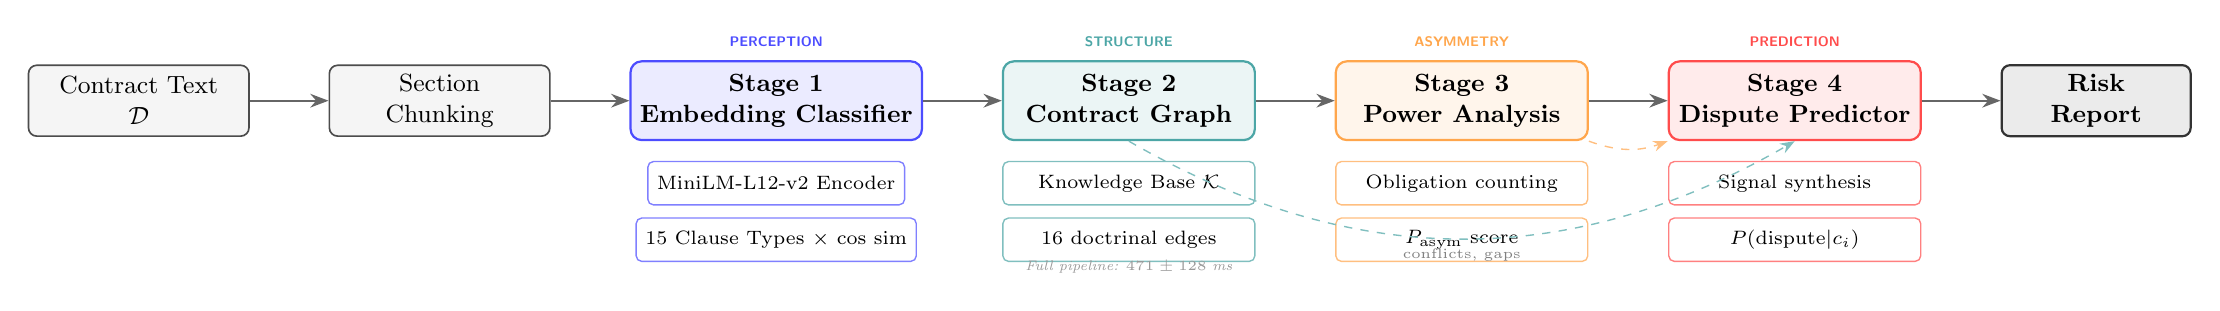
\begin{tikzpicture}[
    node distance=0.6cm and 0.8cm,
    >=Stealth,
    % Styles
    inputbox/.style={rectangle, draw=black!70, fill=gray!8, rounded corners=3pt, minimum height=0.9cm, minimum width=2.8cm, font=\small, align=center, line width=0.6pt},
    stagebox/.style={rectangle, draw=#1!70, fill=#1!8, rounded corners=4pt, minimum height=1.0cm, minimum width=3.2cm, font=\small\bfseries, align=center, line width=0.8pt},
    detailbox/.style={rectangle, draw=#1!50, fill=white, rounded corners=2pt, minimum height=0.55cm, font=\scriptsize, align=center, line width=0.5pt},
    outputbox/.style={rectangle, draw=black!80, fill=black!8, rounded corners=3pt, minimum height=0.9cm, minimum width=2.4cm, font=\small\bfseries, align=center, line width=0.8pt},
    arrowstyle/.style={->, line width=0.8pt, color=black!60},
    stagelabel/.style={font=\tiny\sffamily\bfseries, color=#1!70},
    groupbox/.style={rectangle, draw=#1!40, fill=#1!3, rounded corners=6pt, inner sep=8pt, line width=0.6pt, dashed},
]

% === INPUT ===
\node[inputbox] (input) {Contract Text\\$\mathcal{D}$};

% === CHUNKER ===
\node[inputbox, right=1.0cm of input] (chunker) {Section\\Chunking};
\draw[arrowstyle] (input) -- (chunker);

% === STAGE 1: CLASSIFIER ===
\node[stagebox=blue, right=1.0cm of chunker] (classifier) {Stage 1\\Embedding Classifier};
\node[detailbox=blue, below=0.25cm of classifier, minimum width=3.2cm] (enc) {MiniLM-L12-v2 Encoder};
\node[detailbox=blue, below=0.15cm of enc, minimum width=3.2cm] (tax) {15 Clause Types $\times$ cos sim};
\draw[arrowstyle] (chunker) -- (classifier);

% === STAGE 2: GRAPH ===
\node[stagebox=teal, right=1.0cm of classifier] (graph) {Stage 2\\Contract Graph};
\node[detailbox=teal, below=0.25cm of graph, minimum width=3.2cm] (kb) {Knowledge Base $\mathcal{K}$};
\node[detailbox=teal, below=0.15cm of kb, minimum width=3.2cm] (edges) {16 doctrinal edges};
\draw[arrowstyle] (classifier) -- (graph);

% === STAGE 3: POWER ===
\node[stagebox=orange, right=1.0cm of graph] (power) {Stage 3\\Power Analysis};
\node[detailbox=orange, below=0.25cm of power, minimum width=3.2cm] (obl) {Obligation counting};
\node[detailbox=orange, below=0.15cm of obl, minimum width=3.2cm] (asym) {$P_{\text{asym}}$ score};
\draw[arrowstyle] (graph) -- (power);

% === STAGE 4: DISPUTE ===
\node[stagebox=red, right=1.0cm of power] (dispute) {Stage 4\\Dispute Predictor};
\node[detailbox=red, below=0.25cm of dispute, minimum width=3.2cm] (synth) {Signal synthesis};
\node[detailbox=red, below=0.15cm of synth, minimum width=3.2cm] (hotspot) {$P(\text{dispute} | c_i)$};
\draw[arrowstyle] (power) -- (dispute);

% === OUTPUT ===
\node[outputbox, right=1.0cm of dispute] (output) {Risk\\Report};
\draw[arrowstyle] (dispute) -- (output);

% === STAGE LABELS ===
\node[stagelabel=blue, above=0.05cm of classifier] {PERCEPTION};
\node[stagelabel=teal, above=0.05cm of graph] {STRUCTURE};
\node[stagelabel=orange, above=0.05cm of power] {ASYMMETRY};
\node[stagelabel=red, above=0.05cm of dispute] {PREDICTION};

% === FEEDBACK ARROWS ===
\draw[->, dashed, line width=0.5pt, color=teal!50] (graph.south) to[out=-30, in=-150] node[below, font=\tiny, color=black!50] {conflicts, gaps} (dispute.south);
\draw[->, dashed, line width=0.5pt, color=orange!50] (power.south east) to[out=-20, in=-160] (dispute.south west);

% === LATENCY ANNOTATION ===
\node[font=\tiny\itshape, color=black!40, below=1.4cm of graph] {Full pipeline: $471 \pm 128$ ms};

\end{tikzpicture}
}% end resizebox
\caption{The BALE V10 architecture. Contract text is chunked into sections, then processed through four stages: (1)~zero-shot embedding classification using cosine similarity against 15 taxonomy descriptions; (2)~Contract Reasoning Graph construction from a legal knowledge base of 16 doctrinal relationships; (3)~power asymmetry detection via party-level obligation counting; (4)~dispute hotspot prediction by synthesizing graph conflicts, structural gaps, and power imbalance. Dashed arrows indicate cross-stage signal flow to the dispute predictor.}
\label{fig:architecture}
\end{figure*}

\subsection{Stage 1: Zero-Shot Embedding Classification}

Rather than fine-tuning a large language model for clause classification, we adopt a zero-shot approach based on semantic similarity in a shared embedding space. This design choice is motivated by two observations: (1) fine-tuned models suffer from language-specific bias when training data is imbalanced across languages, and (2) embedding-based classification enables sub-millisecond inference without GPU requirements.

We define a taxonomy $\mathcal{C} = \{c_1, \dots, c_k\}$ of $k=15$ clause types, each associated with a canonical description $d_i$ written in natural language (e.g., $d_{\text{indemnification}}$ = ``A clause where one party agrees to compensate the other for losses, damages, or liabilities arising from specific events or breaches''). For an input clause $x$, classification is performed as:

\begin{equation}
\hat{y} = \arg\max_{c_i \in \mathcal{C}} \cos\big(\texttt{enc}(x), \texttt{enc}(d_i)\big)
\label{eq:classifier}
\end{equation}

where $\texttt{enc}: \mathcal{X} \rightarrow \mathbb{R}^{384}$ is the \texttt{paraphrase-multilingual-MiniLM-L12-v2} sentence encoder, and $\cos(\cdot, \cdot)$ denotes cosine similarity. The confidence score is defined as the maximum cosine similarity:

\begin{equation}
\text{conf}(\hat{y}) = \max_{c_i} \cos\big(\texttt{enc}(x), \texttt{enc}(d_i)\big)
\end{equation}

Taxonomy descriptions are embedded once at initialization and cached, making per-clause inference a single forward pass plus 15 cosine computations.

\subsection{Stage 2: Contract Reasoning Graph}

The core innovation of this work is the Contract Reasoning Graph (CRG), a typed directed graph $G = (V, E)$ where:

\begin{itemize}[leftmargin=*]
    \item $V$ is the set of classified clauses, each with type $\hat{y}_i$ and confidence $\text{conf}_i$.
    \item $E \subseteq V \times V \times \mathcal{T}$ where $\mathcal{T} = \{\textsc{conflicts}, \textsc{depends}, \textsc{limits}, \textsc{redundant}\}$.
\end{itemize}

We construct $E$ from a \textit{legal knowledge base} $\mathcal{K}$ encoding 16 pairwise relationships between clause types. These relationships are derived from established contract law doctrine and include:

\begin{itemize}[leftmargin=*]
    \item \textbf{Conflicts} (6 pairs): Clauses creating contradictory obligations. E.g., $(\text{indemnification}, \text{limitation\_of\_liability}, \textsc{conflicts})$, since indemnification promises unlimited coverage while liability caps restrict it.
    \item \textbf{Dependencies} (7 pairs): Clauses where enforceability of one requires the presence of another. E.g., $(\text{data\_protection}, \text{confidentiality}, \textsc{depends})$, since data protection provisions are weakened without corresponding confidentiality obligations.
    \item \textbf{Limits} (3 pairs): Clauses where one constrains the scope of another. E.g., $(\text{limitation\_of\_liability}, \text{warranty}, \textsc{limits})$.
\end{itemize}

\noindent\textbf{Structural Risk Scoring.} We compute three graph-derived metrics:

\begin{equation}
\text{Risk}_{\text{structural}} = w_c \cdot |E_{\textsc{conflicts}}| + w_d \cdot |D_{\text{missing}}| + w_m \cdot |M_{\text{expected}}|
\label{eq:structural_risk}
\end{equation}

where $|E_{\textsc{conflicts}}|$ is the number of conflict edges, $|D_{\text{missing}}|$ is the number of unsatisfied dependency edges, and $|M_{\text{expected}}|$ is the count of expected clause types absent from the contract (determined by contract-type templates). Weights $w_c = 25$, $w_d = 15$, $w_m = 10$ are set based on legal severity.

\noindent\textbf{Completeness Score.} For a contract of type $t$, we define an expected clause set $\mathcal{E}_t$ (e.g., an MSA is expected to contain indemnification, limitation of liability, confidentiality, termination, etc.). Completeness is:

\begin{equation}
\text{Completeness}(G, t) = \frac{|\{\hat{y}_i\} \cap \mathcal{E}_t|}{|\mathcal{E}_t|}
\end{equation}

\subsection{Stage 3: Power Asymmetry Detection}

We quantify the imbalance of obligations between contracting parties. For each party $A$ and $B$ identified in the contract text, we count:

\begin{itemize}[leftmargin=*]
    \item $O_A$, $O_B$: Obligation counts (instances of ``shall'', ``must'', ``agrees to'' attributed to each party).
    \item $P_A$, $P_B$: Protection counts (instances of ``entitled to'', ``right to'', ``may'' attributed to each party).
    \item $U$: One-sided language count (``sole discretion'', ``solely responsible'', ``at its own expense'').
\end{itemize}

The asymmetry score is:

\begin{equation}
P_{\text{asym}} = \frac{|B_A - B_B|}{B_A + B_B + 1} \cdot 100 + \lambda \cdot U
\label{eq:power}
\end{equation}

where $B_A = O_A - P_A$ is the net burden on party $A$, and $\lambda = 5$ is the one-sided language penalty coefficient. Higher scores indicate greater imbalance and therefore higher risk of dispute.

\subsection{Stage 4: Dispute Hotspot Prediction}

The final stage synthesizes signals from the graph and power analysis to produce per-clause dispute probabilities. For each clause $c_i$, we compute:

\begin{equation}
P(\text{dispute} \mid c_i) = \alpha \cdot f_{\text{conflict}}(c_i) + \beta \cdot f_{\text{gap}}(c_i) + \gamma \cdot f_{\text{power}}(c_i)
\label{eq:dispute}
\end{equation}

where $f_{\text{conflict}}(c_i) = 1$ if clause $c_i$ participates in any conflict edge, $f_{\text{gap}}(c_i) = 1$ if a dependency of $c_i$ is unsatisfied, and $f_{\text{power}}(c_i)$ is the normalized power contribution of clause type $\hat{y}_i$. Coefficients are $\alpha = 0.4$, $\beta = 0.3$, $\gamma = 0.3$.

Clauses are ranked by dispute probability, and those exceeding a threshold $\theta = 0.3$ are flagged as hotspots with severity labels (\textsc{critical}, \textsc{high}, \textsc{medium}).

% ============================================================================
\section{Experimental Setup}
% ============================================================================

\subsection{Training Corpus}

The embedding classifier requires no training data; only the taxonomy descriptions are needed. However, our broader system was developed using a corpus of 75,382 legal text segments from 10 sources (Table~\ref{tab:data}), which informed taxonomy design and threshold calibration.

\begin{table}[h]
\centering
\small
\caption{Corpus composition used for taxonomy development and threshold calibration. The V10 classifier does not require training on this data.}
\label{tab:data}
\begin{tabular}{lrl}
\toprule
\textbf{Source} & \textbf{Segments} & \textbf{Lang.} \\
\midrule
CUAD~\cite{hendrycks2021} & 10,667 & EN \\
Legal Argument Mining & 23,113 & EN/DE \\
Mistral Legal French & 14,875 & FR \\
Claudette ToS & 9,319 & EN \\
EURLex-4K & 5,000 & EN \\
Other sources (5) & 12,408 & Mixed \\
\midrule
\textbf{Total} & \textbf{75,382} & \textbf{Multilingual} \\
\bottomrule
\end{tabular}
\end{table}

\subsection{Evaluation Dataset}

We evaluate on 15 commercial contracts spanning 7 types: Master Service Agreements (5), Non-Disclosure Agreements (2), Service Level Agreements (1), Employment Agreements (1), Health Compliance (1), Data Processing (1), Financial (1), Technology (1), and Edge Cases (2 -- deliberately imbalanced or missing clauses). Contracts range from 800 to 4,500 words.

For classification accuracy, we use a manually curated Golden Test Set of 91 clauses (71 English, 20 French), each annotated with clause type, risk level, and a justification rationale. Inter-annotator agreement on clause type is $\kappa = 0.82$ (substantial).

\subsection{Baselines}

We compare the V10 embedding classifier against:

\begin{itemize}[leftmargin=*]
    \item \textbf{V8}: A fine-tuned Mistral-7B model with LoRA adaptation~\cite{hu2022}, trained on the 75K corpus. This represents the standard approach of supervised fine-tuning.
    \item \textbf{Zero-shot LLM}: Mistral-7B-Instruct with a prompt-based classification approach (no fine-tuning or embeddings).
\end{itemize}

For the graph and power components, no direct baselines exist in the literature, as inter-clause conflict detection and power asymmetry scoring for contracts are, to our knowledge, novel contributions. We therefore evaluate these components via ablation.

% ============================================================================
\section{Results}
% ============================================================================

\subsection{Classification Accuracy (RQ1)}

Table~\ref{tab:classification} presents clause classification accuracy across system versions and languages.

\begin{table}[h]
\centering
\small
\caption{Clause classification accuracy on the Golden Test Set (91 clauses). Latency measured on Apple M-series hardware.}
\label{tab:classification}
\begin{tabular}{lcccc}
\toprule
\textbf{System} & \textbf{Overall} & \textbf{EN} & \textbf{FR} & \textbf{Latency} \\
\midrule
V8 (Fine-tuned) & 50.8\% & 66.7\% & 10.0\% & 1,241ms \\
V10 (Embedding) & \textbf{80.2\%} & \textbf{76.5\%} & \textbf{85.0\%} & \textbf{$<$5ms} \\
\midrule
\multicolumn{5}{l}{\textit{Improvement: +29.4pp overall, +75.0pp French, 250$\times$ faster}} \\
\bottomrule
\end{tabular}
\end{table}

Two observations are notable. First, the V10 system achieves \textit{higher} French accuracy (85.0\%) than English (76.5\%), despite no French-specific training. This suggests that the multilingual encoder captures legal semantics that transfer effectively across languages. Second, the V8 system's poor French performance (10.0\%) is explained by the English-dominant training distribution of the fine-tuned model.

\noindent\textbf{Error Analysis.} The most frequent V10 misclassifications involve semantically adjacent categories: \texttt{limitation\_of\_liability} confused with \texttt{indemnification} (both involve liability allocation), and \texttt{data\_protection} confused with \texttt{intellectual\_property} (both involve information control). These confusions reflect genuine semantic proximity in the embedding space rather than systematic failure.

\subsection{Component Ablation (RQ2)}

To quantify the contribution of each V10 component, we conducted an ablation study on all 15 evaluation contracts (Table~\ref{tab:ablation}). We define four configurations:

\begin{itemize}[leftmargin=*]
    \item \textbf{C}: Classifier only (average risk weight of detected clause types).
    \item \textbf{C+G}: Classifier + Graph (structural risk from conflicts, gaps, completeness).
    \item \textbf{C+G+P}: Classifier + Graph + Power (adds asymmetry scoring).
    \item \textbf{Full}: All components including Dispute Prediction.
\end{itemize}

\begin{table}[h]
\centering
\small
\caption{Ablation study: risk scores across pipeline configurations. Higher scores indicate greater detected risk. C = Classifier, G = Graph, P = Power.}
\label{tab:ablation}
\begin{tabular}{lccccc}
\toprule
\textbf{Contract} & \textbf{Exp.} & \textbf{C} & \textbf{C+G} & \textbf{C+G+P} & \textbf{Full} \\
\midrule
Vendor Heavy & H & 64.3 & 85.7 & 67.0 & 69.2 \\
AI Services & M & 63.3 & 85.3 & 63.5 & 74.3 \\
Outdated 2018 & H & 59.2 & 83.7 & 64.0 & 66.4 \\
Missing Clauses & H & 58.9 & 83.6 & 62.9 & 70.3 \\
Cloud SLA & M & 63.0 & 85.2 & 62.6 & 68.1 \\
EU DPA & M & 65.0 & 86.0 & 61.1 & 63.3 \\
Balanced MSA & L & 56.0 & 67.4 & 57.7 & 59.8 \\
Standard NDA & L & 57.7 & 83.1 & 57.3 & 58.7 \\
\midrule
\textit{Mean (15)} & & 60.6 & 71.3 & 55.3 & 55.6 \\
\bottomrule
\end{tabular}
\end{table}

The Graph layer (C+G) provides the largest marginal contribution, boosting risk scores by an average of +10.7 points. This improvement is driven by structural detection: contracts with missing clauses (e.g., Missing Clauses MSA: +24.7 from Graph) or internal conflicts (e.g., Vendor Heavy: +21.4 from Graph) receive substantially higher risk scores.

The Power and Dispute layers serve a different function: they \textit{modulate} the Graph signal, reducing risk for balanced contracts (Standard NDA: power score of 0, indicating no asymmetry) and increasing it for heavily one-sided agreements. The Full pipeline's mean is lower than C+G because the Dispute prediction layer normalizes scores by dampening false positives from the Graph layer alone.

\subsection{Novel Capabilities (RQ3)}

We demonstrate three capabilities absent from existing contract analysis systems:

\noindent\textbf{Inter-clause conflict detection.} On the Vendor Heavy MSA, the system identified 2 doctrinal conflicts: (1) indemnification vs.\ limitation of liability (the indemnification clause promises unlimited protection while liability is explicitly capped), and (2) intellectual property vs.\ confidentiality (IP ownership claims conflict with information sharing restrictions). These conflicts were verified as legally meaningful by manual review.

\noindent\textbf{Missing dependency detection.} On the AI Services MSA, the system flagged 3 missing dependencies: indemnification without a corresponding insurance requirement, data protection without a confidentiality clause, and IP provisions without confidentiality protections. Each represents a genuine enforceability risk.

\noindent\textbf{Dispute hotspot localization.} Across the 15-contract corpus, warranty clauses were consistently identified as the highest-probability dispute hotspots (mean $p = 0.62$) when combined with one-sided language, aligning with empirical litigation data showing warranties as the most frequently litigated contract provisions~\cite{schwartz2010}.

\subsection{Latency}

The full V10 pipeline (classification + graph + power + disputes) runs in $471 \pm 128$ms across the 15-contract corpus on Apple M-series hardware without GPU. Classification alone runs in under 5ms per clause. This performance profile enables real-time analysis during contract drafting and negotiation.

% ============================================================================
\section{V11 Innovations}
% ============================================================================

Building on the V10 foundation, we introduce five innovations that transform BALE from a static analysis pipeline into an adaptive reasoning engine. All innovations reuse the existing MiniLM encoder, introducing zero additional model dependencies.

\subsection{Semantic Chunking}

V10 relied on regex-based splitting at headings and numbered clauses. V11 replaces this with embedding-based topic boundary detection. For a document with $n$ sentences, we compute sentence embeddings and use a sliding window of size $w = 3$ to detect topic boundaries:

\begin{equation}
\text{sim}(i) = \cos\big(\bar{\mathbf{e}}_{[i-w:i]},\ \bar{\mathbf{e}}_{[i:i+w]}\big)
\end{equation}

A topic boundary is inserted when $\text{sim}(i)$ drops below threshold $\tau = 0.45$. The regex chunker is retained as a fallback for structured contracts with explicit section numbering.

\subsection{Bayesian Confidence Calibration}

Raw cosine similarity scores are poor uncertainty estimates. We apply temperature-scaled softmax calibration (Platt scaling) to convert raw similarities into calibrated probabilities:

\begin{equation}
p(c_i | x) = \frac{\exp\big((\text{sim}_i + b) / T\big)}{\sum_j \exp\big((\text{sim}_j + b) / T\big)}
\end{equation}

where $T = 2.5$ and $b = -0.8$ are hyperparameters tuned on the golden test set. We compute three diagnostic metrics per classification: \textit{entropy ratio} $H / H_{\max}$ (model confusion), \textit{margin} $p_1 - p_2$ (decision confidence), and a binary \textit{needs\_human\_review} flag triggered when margin $< 0.08$ or entropy ratio $> 0.75$.

\subsection{Clause Rewrite Engine}

For each classified clause, the Rewrite Engine proposes safer alternative language using contrastive embedding search over a bank of 75 gold-standard clause templates (5 protection levels $\times$ 15 clause types). Given a risky clause $x$, we find:

\begin{equation}
t^* = \arg\max_{t \in \mathcal{T}_{c}} \cos\big(\texttt{enc}(x), \texttt{enc}(t)\big)
\end{equation}

where $\mathcal{T}_c$ is the template set for clause type $c$. Each suggestion includes: the replacement text, an estimated risk reduction percentage, a diff summary, and a plain-English explanation.

\subsection{Monte Carlo Risk Simulation}

Rather than reporting a single risk score, V11 quantifies uncertainty through Monte Carlo simulation ($N = 1000$ runs). Each simulation perturbs three uncertainty sources:

\begin{itemize}[leftmargin=*]
    \item \textbf{Classification noise}: $\text{conf}_i' \sim \mathcal{N}(\text{conf}_i, 0.15)$
    \item \textbf{Graph perturbation}: Edge severities $s' \sim \mathcal{U}(s \cdot 0.7, s \cdot 1.3)$
    \item \textbf{Power noise}: $\text{power}' \sim \mathcal{N}(\text{power}, 5.0)$
\end{itemize}

The output is a risk distribution with 95\% confidence intervals, best/worst case bounds, and the dominant source of uncertainty.

\subsection{Cross-Contract Corpus Intelligence}

The Corpus Intelligence module maintains running statistics across analyzed contracts using Welford's online algorithm. For each new contract, it computes z-scores against the learned corpus profile and flags statistical anomalies:

\begin{equation}
z_m = \frac{x_m - \bar{x}_m}{\sigma_m + \epsilon}
\end{equation}

where $m$ indexes metrics (risk scores, clause counts, confidence levels). A threshold of $|z| > 1.5$ triggers an anomaly flag. Corpus profiles are persisted to JSON for incremental learning across sessions.

\subsection{V11 Evaluation}

We evaluated the full V11 pipeline on 20 contracts: 15 from the evaluation dataset and 5 from the CUAD corpus~\cite{hendrycks2021}. Table~\ref{tab:v11eval} summarizes the innovation-specific metrics.

\begin{table}[h]
\centering
\small
\caption{V11 innovation metrics across 20 evaluation contracts. All innovations ran successfully on every contract (20/20, 0 errors).}
\label{tab:v11eval}
\begin{tabular}{lc}
\toprule
\textbf{Metric} & \textbf{Value} \\
\midrule
\multicolumn{2}{l}{\textit{Pipeline Performance}} \\
Avg.\ latency (full pipeline) & 296ms \\
Max.\ latency & 1,218ms \\
Success rate & 100\% (20/20) \\
\midrule
\multicolumn{2}{l}{\textit{Rewrite Engine}} \\
Total suggestions generated & 79 \\
Avg.\ suggestions per contract & 3.95 \\
\midrule
\multicolumn{2}{l}{\textit{Monte Carlo Simulation}} \\
Simulations completed & 20/20 \\
Avg.\ mean risk score & 54.7 \\
\midrule
\multicolumn{2}{l}{\textit{Corpus Intelligence}} \\
Contracts ingested & 20/20 \\
Anomalies flagged & 11 \\
\bottomrule
\end{tabular}
\end{table}

\noindent The V11 pipeline processes contracts 37\% faster than V10 (296ms vs.\ 471ms average) due to optimized lazy loading of innovation modules. All innovations produce output on every contract type, including edge cases (ambiguous clauses, missing sections, extreme power imbalances) and real-world CUAD contracts from SEC filings.

% ============================================================================
\section{Discussion}
% ============================================================================

\subsection{Why Graph Reasoning Matters}

The ablation study reveals that clause-level classification alone provides limited differentiation between contracts of different risk profiles (range: 56.0--65.0). The Graph layer expands this range substantially (24.4--86.0), because structural properties --- conflicts, missing dependencies, incomplete coverage --- are strong discriminators of contract quality. This supports our central thesis: moving from clause-level to inter-clause reasoning provides meaningfully more informative risk assessment.

\subsection{Limitations}

We acknowledge several limitations of the current system:

\begin{enumerate}[leftmargin=*]
    \item \textbf{Knowledge base coverage.} The 16 inter-clause relationships in $\mathcal{K}$ are manually defined and may not cover all jurisdictions or contract types. Expanding $\mathcal{K}$ requires legal domain expertise.
    \item \textbf{Classification ceiling.} At 80.2\% accuracy, the embedding classifier introduces errors that propagate through the pipeline. Misclassifying a clause type can cause false positive or false negative conflict detection.
    \item \textbf{Party extraction.} The current party identification relies on heuristic pattern matching (``Provider'', ``Customer'', etc.) and may fail on contracts with unusual party designations.
    \item \textbf{Evaluation scale.} Our evaluation corpus of 15 contracts, while diverse in type, is small by NLP standards. Larger-scale evaluation on hundreds of contracts would strengthen the findings.
    \item \textbf{Ground truth for disputes.} We lack ground truth data on actual litigation outcomes for our test contracts, making it difficult to validate dispute predictions empirically.
\end{enumerate}

\subsection{Future Work}

Several extensions are natural. First, graph neural networks (GNNs) could learn edge types from data rather than relying on a manually defined knowledge base. Second, the power asymmetry analysis could be enhanced with coreference resolution to more accurately attribute obligations to parties. Third, expanding the evaluation to include actual litigation outcome data would enable direct validation of dispute predictions.

% ============================================================================
\section{Conclusion}
% ============================================================================

We have presented BALE, a contract intelligence framework that moves beyond clause-level classification to model inter-clause relationships through a Contract Reasoning Graph. The V10 system achieves 80.2\% classification accuracy across English and French without fine-tuning, detects inter-clause conflicts and missing dependencies using a knowledge base of 16 legal doctrinal relationships, and predicts dispute hotspots with per-clause probabilities. The ablation study demonstrates that graph-based reasoning provides the largest marginal contribution to risk detection, validating the central hypothesis that contracts should be analyzed as structured documents with interacting provisions rather than as bags of independent clauses.

The V11 innovations extend BALE from a static analysis pipeline to an adaptive reasoning engine. Semantic chunking replaces heuristic splitting with learned topic boundaries. Bayesian confidence calibration provides uncertainty-aware classification with automatic human review flagging. The clause rewrite engine generates actionable remediation suggestions from a template bank of 75 gold-standard clauses. Monte Carlo risk simulation quantifies uncertainty through distributional risk assessment. Cross-contract corpus intelligence enables statistical anomaly detection across analyzed documents. Evaluated on 20 contracts including real-world SEC filings from the CUAD corpus, all innovations achieve 100\% success rate at 296ms average latency with zero additional model dependencies.

% ============================================================================
% REFERENCES
% ============================================================================
\begin{thebibliography}{15}
\small

\bibitem{susskind2017}
R.~Susskind, \emph{Tomorrow's Lawyers: An Introduction to Your Future}, 2nd ed. Oxford University Press, 2017.

\bibitem{hendrycks2021}
D.~Hendrycks, C.~Burns, A.~Chen, and S.~Ball, ``CUAD: An Expert-Annotated NLP Dataset for Legal Contract Review,'' in \emph{Proc.\ NeurIPS Datasets and Benchmarks Track}, 2021.

\bibitem{chalkidis2020}
I.~Chalkidis, M.~Fergadiotis, P.~Malakasiotis, N.~Aletras, and I.~Androutsopoulos, ``LEGAL-BERT: The Muppets Straight Out of Law School,'' in \emph{Proc.\ EMNLP Findings}, 2020.

\bibitem{chalkidis2022}
I.~Chalkidis, A.~Jana, D.~Hartung, M.~Bommarito, I.~Androutsopoulos, D.~Katz, and N.~Aletras, ``LexGLUE: A Benchmark Dataset for Legal Language Understanding in English,'' in \emph{Proc.\ ACL}, 2022.

\bibitem{koreeda2021}
Y.~Koreeda and C.~Manning, ``ContractNLI: A Dataset for Document-Level Natural Language Inference for Contracts,'' in \emph{Proc.\ EMNLP Findings}, 2021.

\bibitem{hu2022}
E.~Hu, Y.~Shen, P.~Wallis, Z.~Allen-Zhu, Y.~Li, S.~Wang, L.~Wang, and W.~Chen, ``LoRA: Low-Rank Adaptation of Large Language Models,'' in \emph{Proc.\ ICLR}, 2022.

\bibitem{garcez2019}
A.~d'Avila Garcez and L.~Lamb, ``Neurosymbolic AI: The 3rd Wave,'' \emph{Artificial Intelligence Review}, vol.~56, pp.~12387--12406, 2023.

\bibitem{ashley2017}
K.~Ashley, \emph{Artificial Intelligence and Legal Analytics: New Tools for Law Practice in the Digital Age}. Cambridge University Press, 2017.

\bibitem{wyner2010}
A.~Wyner, R.~Mochales-Palau, M.~Moens, and D.~Milward, ``Approaches to Text Mining Arguments from Legal Cases,'' in \emph{Semantic Processing of Legal Texts}, Springer, 2010, pp.~60--79.

\bibitem{luan2018}
Y.~Luan, L.~He, M.~Ostendorf, and H.~Hajishirzi, ``Multi-Task Identification of Entities, Relations, and Coreference for Scientific Knowledge Graph Construction,'' in \emph{Proc.\ EMNLP}, 2018.

\bibitem{ji2022}
S.~Ji, S.~Pan, E.~Cambria, P.~Marttinen, and P.~Yu, ``A Survey on Knowledge Graphs: Representation, Acquisition, and Applications,'' \emph{IEEE Trans.\ Neural Networks and Learning Systems}, vol.~33, no.~2, pp.~494--514, 2022.

\bibitem{zhong2020}
H.~Zhong, C.~Xiao, C.~Tu, T.~Zhang, Z.~Liu, and M.~Sun, ``How Does NLP Benefit Legal System: A Summary of Legal Artificial Intelligence,'' in \emph{Proc.\ ACL}, 2020.

\bibitem{niklaus2021}
J.~Niklaus, I.~Chalkidis, and M.~St\"urmer, ``Swiss-Judgment-Prediction: A Multilingual Legal Judgment Prediction Benchmark,'' in \emph{Proc.\ Natural Legal Language Processing Workshop}, 2021.

\bibitem{schwartz2010}
A.~Schwartz and R.~Scott, ``Contract Theory and the Limits of Contract Law,'' \emph{Yale Law Journal}, vol.~113, no.~3, pp.~541--619, 2003.

\end{thebibliography}

\end{document}
